\documentclass[11pt]{beamer}
\usepackage{amsmath, amsfonts, amscd, amssymb, amsthm, tikz,pgfplots}
\setbeamertemplate{navigation symbols}{}

\usepackage{caption}

\usetheme{eaperry}


\usepackage{changepage}
\usepackage{array}
%\usepackage{multirow}
%\usepackage{float}
%\usepackage{tabu}
%\usepackage{threeparttable}
%\usepackage{threeparttablex}
%\usepackage[normalem]{ulem}
%\usepackage{makecell}
%\usepackage{xcolor}


\bibliographystyle{aer}
\usepackage{natbib}

\title{Data Exploration}
\subtitle{Assessing the Modified Alonso-Muth-Mills Model}
\institute{Spellman Program}
\author{Evan Perry}
\date{July 20, 2021}

\begin{document}

\maketitlepage

\begin{frame}{Review}

\begin{exampleblock}{\large\textbf{Research Question}}
What characteristics of urban neighborhoods relate to the number of certified green commercial buildings?
\end{exampleblock}

\vfill
Previously,
\begin{itemize}
	\item Modified the Alonso-Muth-Mills model to describe where green buildings are built
	\item Data background, data cleaning, descriptive statistics
	\item Evaluating the model?
\end{itemize}

\end{frame}


\begin{frame}{Outline}

\begin{block}{\textbf{Today's Goal}}
Spend some time evaluating the modified Alonso-Muth-Mills model: what works, what doesn't, and what do we want out of our model?
\end{block}

	\tableofcontents[hideallsubsections]
\end{frame}

\newsection{Revisiting the Alonso-Muth-Mills Model}{\textit{Modifications \& More}}

\begin{frame}{The Modified AMM}

\begin{figure}
\centering
\caption{Bid-Rent Curves with a Fixed Premium}
\begin{tikzpicture}
\begin{axis}[
	axis lines = left,
	ticks=none,
    ylabel = {Price of Land ($p_L$)},
    xlabel = {Distance from City Center ($x$)},
    xmin=0, xmax=10,
    ymin=0, ymax=15,
	every axis plot/.append style={ultra thick}
]
\addplot[
	domain = 0.1:10,
	samples=100,
	color=EAPred
]{(1/(100000*(10-0.2*x)^(-1)))^(1/0.4) * (0.6/(0.4*10))^(0.6/0.4) * 
       (0.4/(1))^((1)/0.4)*(50000*(10 - 0.2*x) - 10000 - 265750)^((1)/0.4)};
\addplot[
	domain = 0.1:10,
	samples=100,
	color=EAPgreen
]{(1/(100000*(10-0.2*x)^(-1)))^(1/0.4) * (0.6/(0.4*20))^(0.6/0.4) * 
       (0.4/(1))^((1)/0.4)*( 
       (50000*(1/100000)*(10 - 0.2*x)^(1+1) + 8.5)*100000*(10-0.2*x)^(-1)
         - 10000 - 265750)^((1)/0.4)};
\end{axis}
\node[EAPgreen] at (7.2,1.2) {$p_L^G$};
\node[EAPred] at (7.2,0.6) {$p_L^N$};
\draw[dashed]  (3,0) -- (3,5.4);
\node[EAPred] at (1.5, 5) {\footnotesize Non-Green};
\node[EAPgreen] at (4.5, 5) {\footnotesize Green};
%\node at (5.1, 5) {\footnotesize $\Delta p KWH > \Delta \psi \rho$};
\end{tikzpicture}
\end{figure}

\end{frame}


\begin{frame}{Another Modification }

\begin{figure}
\centering
\caption{Bid-Rent Curves with a Social Premium}
\begin{tikzpicture}
\begin{axis}[
	axis lines = left,
	ticks=none,
    ylabel = {Price of Land ($p_L$)},
    xlabel = {Distance from City Center ($x$)},
    xmin=0, xmax=10,
    ymin=0, ymax=19,
	every axis plot/.append style={ultra thick}
]
\addplot[
	domain = 0.1:10,
	samples=100,
	color=EAPred
]{(1/(100000*(10-0.2*x)^(-1)))^(1/0.4) * (0.6/(0.4*10))^(0.6/0.4) * 
       (0.4/(1))^((1)/0.4)*(50000*(10 - 0.2*x) - 10000 - 265750)^((1)/0.4)};
\addplot[
	domain = 0.1:10,
	samples=100,
	color=EAPgreen
]{(1/(100000*(10-0.2*x)^(-1)))^(1/0.4) * (0.6/(0.4*20))^(0.6/0.4) * 
       (0.4/(1))^((1)/0.4)*( 
       (50000*(1/100000)*(10 - 0.2*x )^(1+1) + 7 + 0.0007*(x -10)^4)*100000*(10-0.2*x)^(-1)
         - 10000 - 265750)^((1)/0.4)};
\end{axis}
\node[EAPgreen] at (7.2,1) {$p_L^G$};
\node[EAPred] at (7.2,0.4) {$p_L^N$};
\draw[dashed]  (1.2,0) -- (1.2,5.4);
\draw[dashed] (4.5,0) -- (4.5, 5.4);
\node[EAPred] at (3, 5) {\footnotesize Non-Green};
\node[EAPgreen] at (5.5, 5) {\footnotesize Green};
\node[EAPgreen] at (.6,5) {\footnotesize Green};
%\node at (5.1, 5) {\footnotesize $\Delta p KWH > \Delta \psi \rho$};
\end{tikzpicture}
\end{figure}

\end{frame}


\newsection{Evidence for the Model}{\textit{Are the data consistent with the theory?}}


\begin{frame}{Initial Mapping}
\begin{figure}
\caption{Green Building Counts, Indianapolis}
\centering
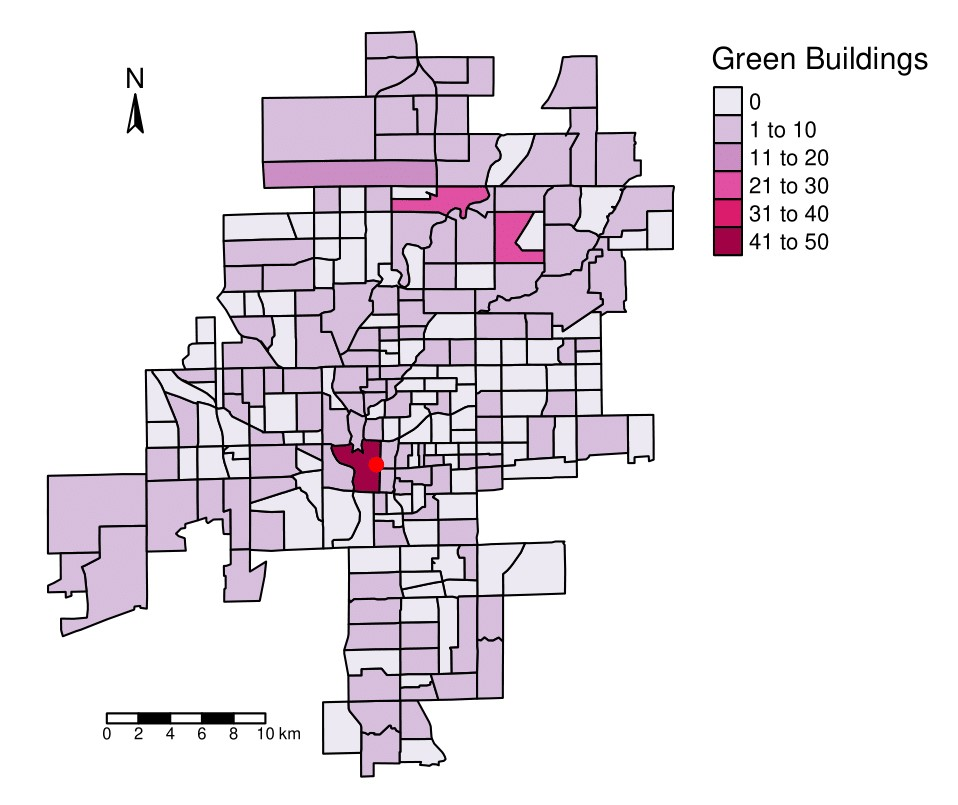
\includegraphics[width=0.7\textwidth]{indCounts-1.jpg}
\end{figure}
\end{frame}

\begin{frame}{Separating by Type}
\centering
\captionof{figure}{Green Building Locations by Type}
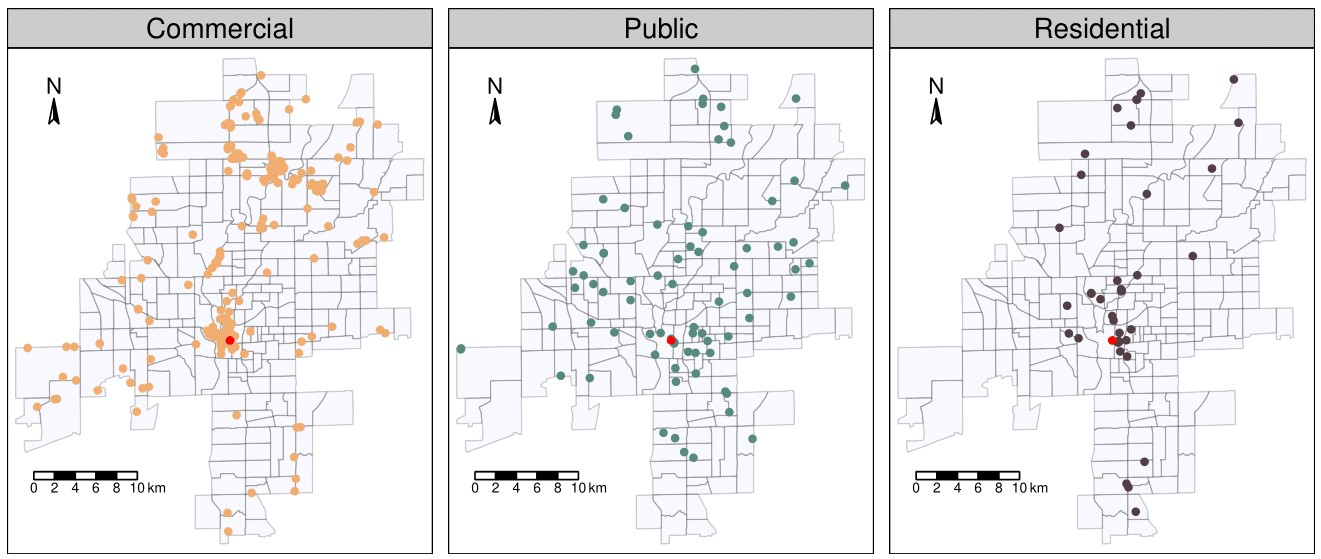
\includegraphics[width=\textwidth]{indPoints-1.jpg}
\end{frame}


\begin{frame}{Linearizing the City}

\begin{figure}
\caption{Green Buildings' Distance from the City Center, Indianapolis}
\centering
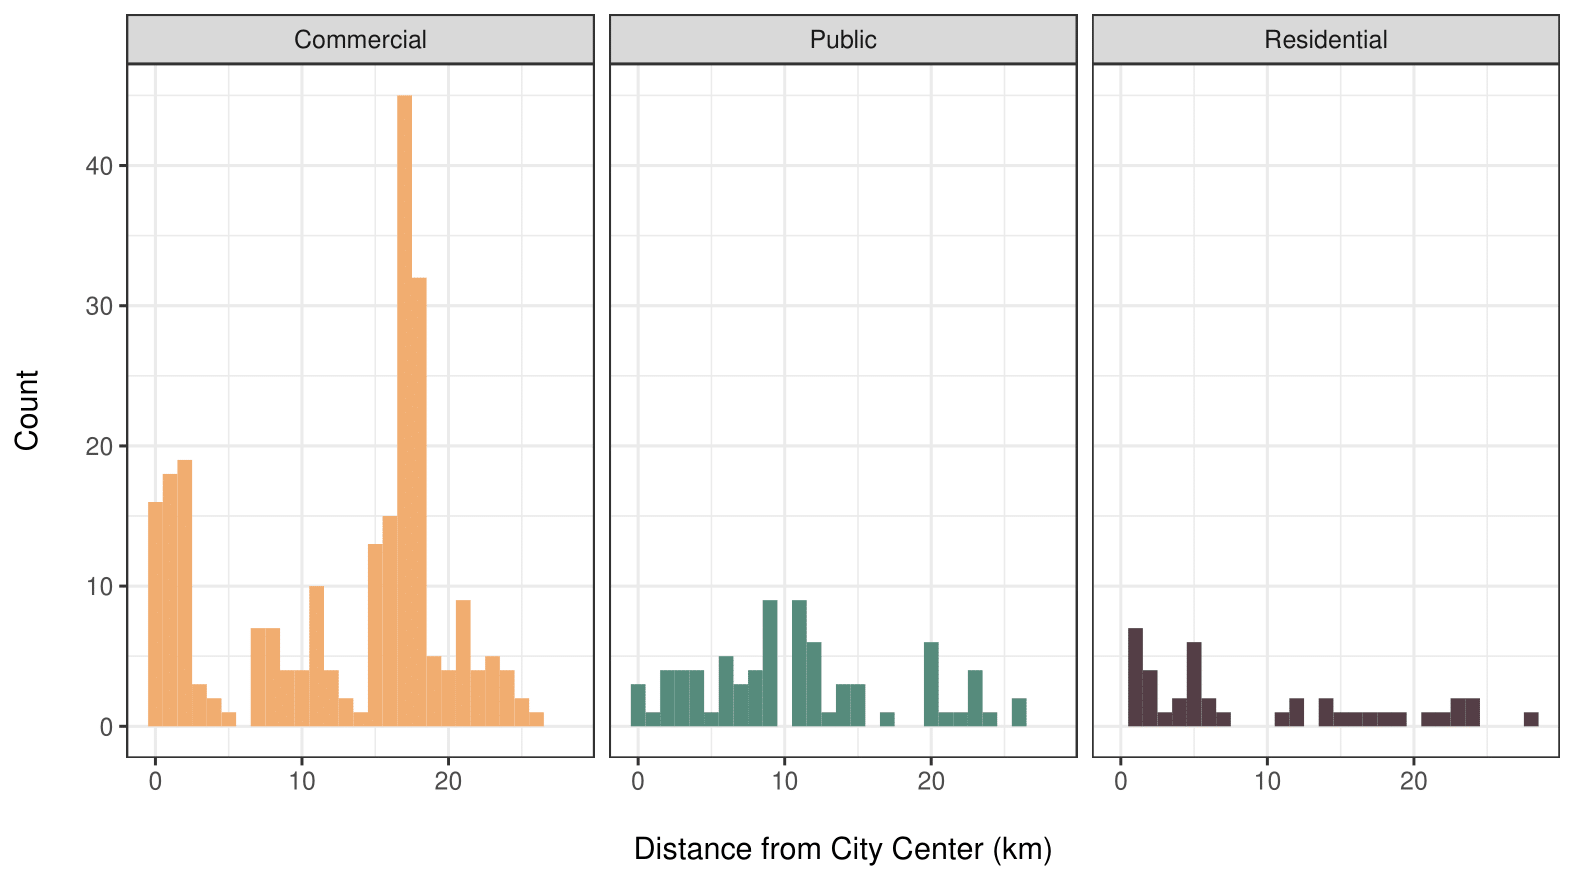
\includegraphics[width=\textwidth]{indHist-1.png}
\end{figure}

\end{frame}


\begin{frame}{Evidence of the Three Zones}

\begin{figure}
\caption{Distribution of Green Buildings by Type, Indianapolis}
\centering
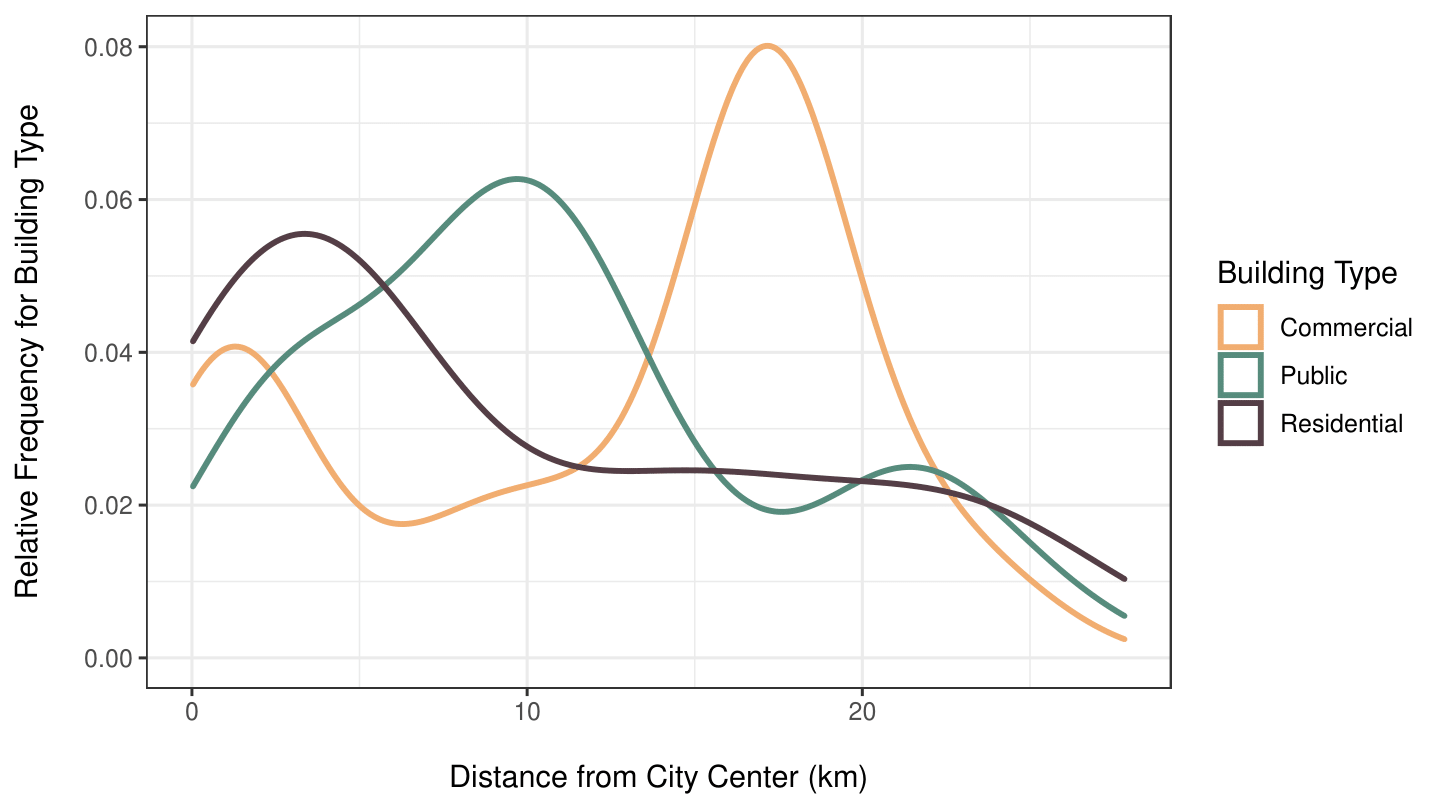
\includegraphics[width=\textwidth]{indDensity-1.png}
\end{figure}

\end{frame}


\begin{frame}{Consistent Cities}

\begin{figure}
\caption{Distribution of Commercial Green Buildings, Four Cities}
\centering
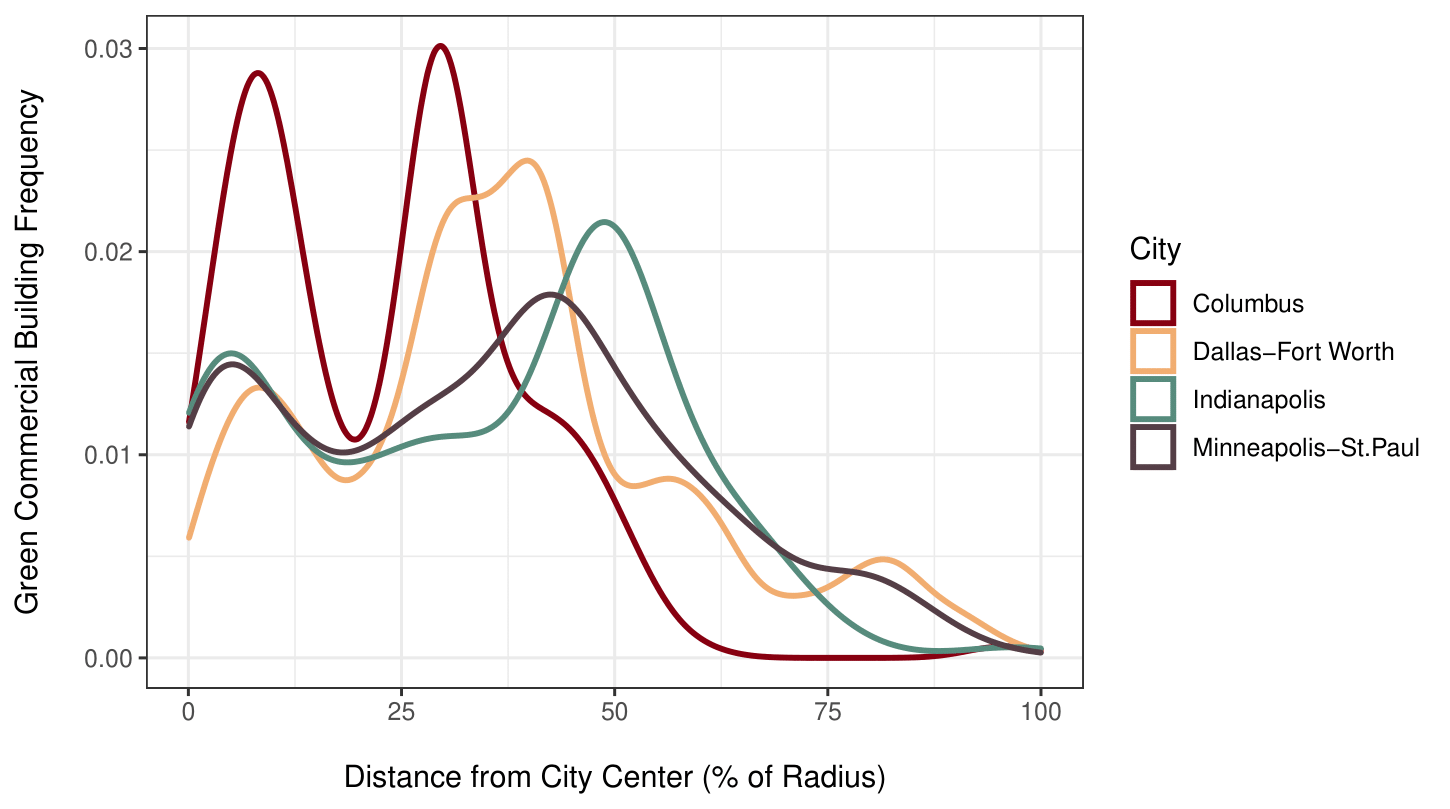
\includegraphics[width=\textwidth]{goodCities-1.png}
\end{figure}

\end{frame}


\begin{frame}{Inconsistent Cities}

\begin{figure}
\caption{Distribution of Commercial Green Buildings, Four Other Cities}
\centering
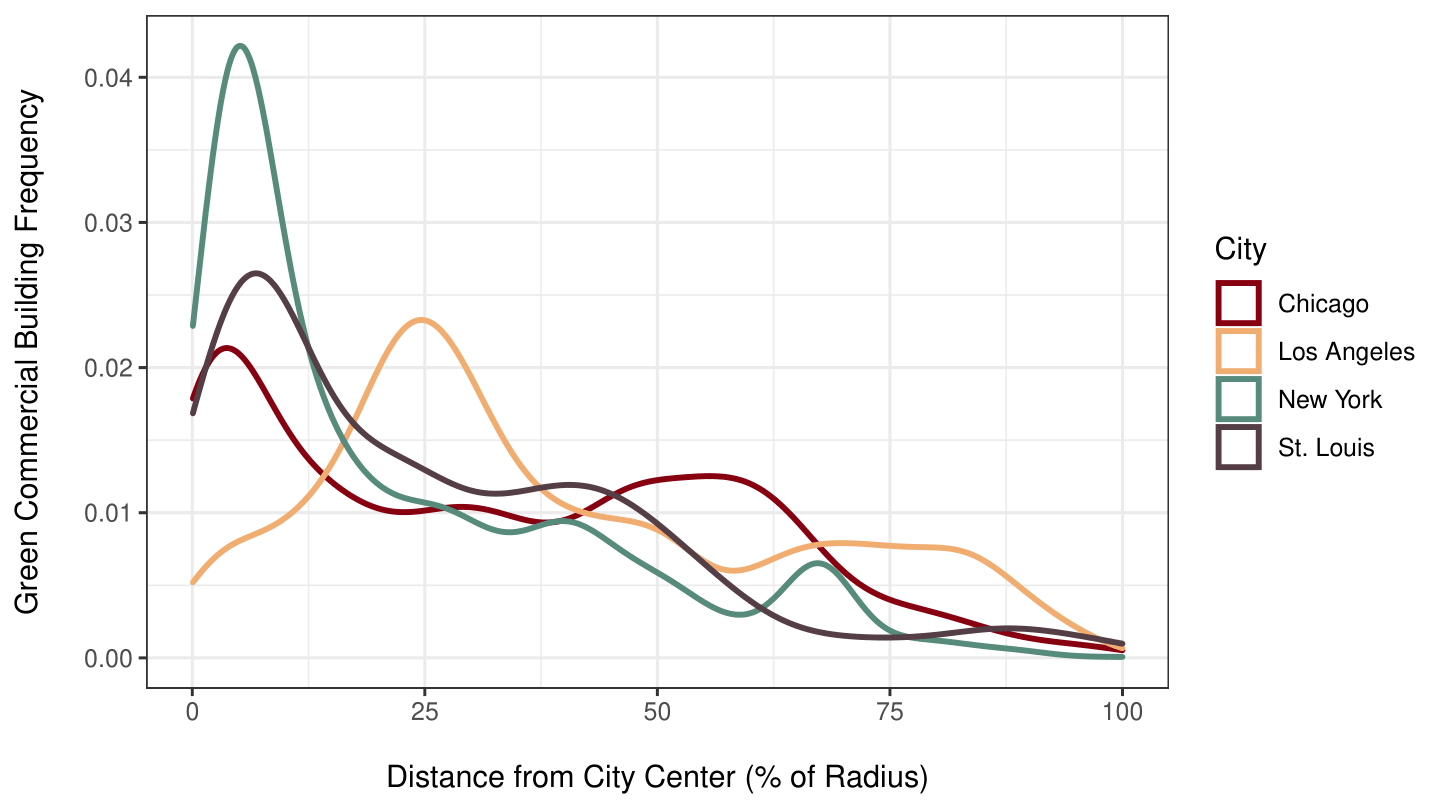
\includegraphics[width=\textwidth]{badCities-1.png}
\end{figure}

\end{frame}


\newsection{Alternative Explanations}{\textit{Incorporating Census Data}}

\begin{frame}
\begin{columns}
\begin{column}{0.48\textwidth}
\begin{figure}
\caption{Commercial Green Building Counts, Indianapolis}
\centering
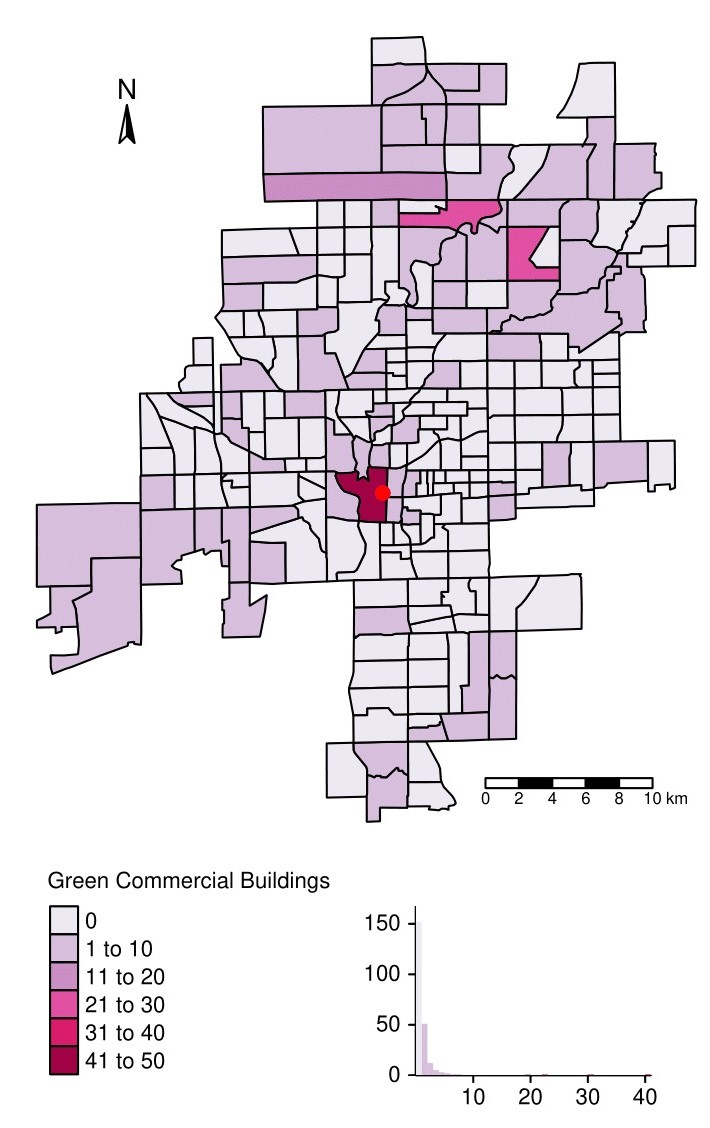
\includegraphics[width=.8\textwidth]{indComCounts-1.jpg}
\end{figure}
\end{column}
\begin{column}{0.48\textwidth}
\begin{figure}
\caption{Median Household Income, Indianapolis}
\centering
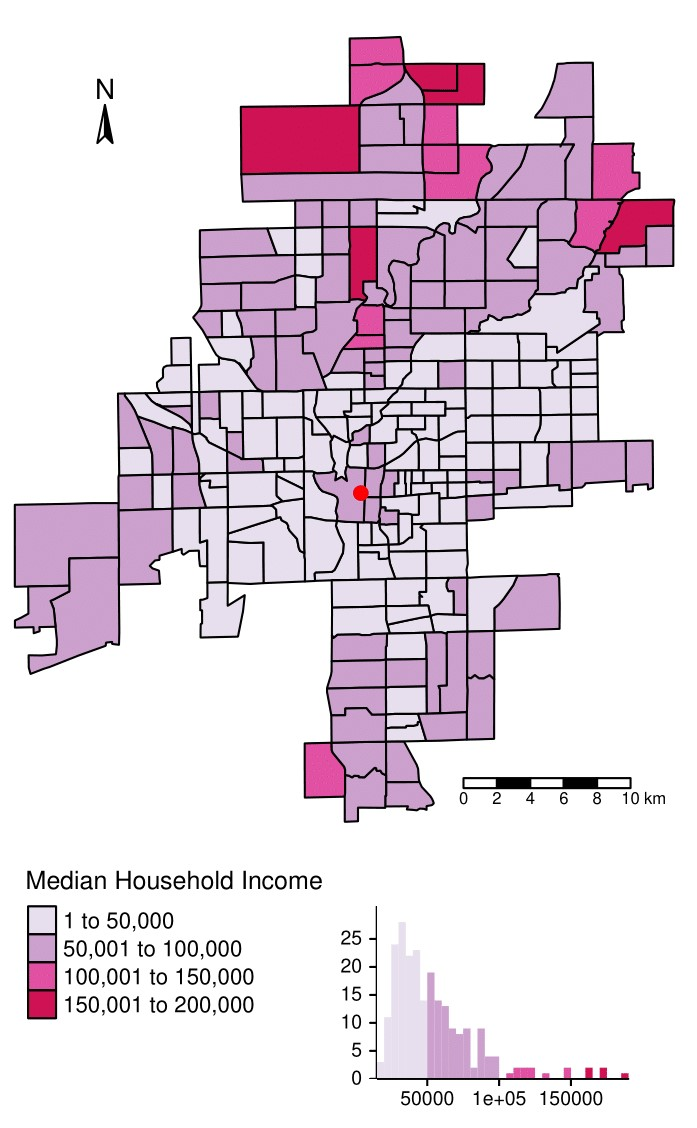
\includegraphics[width=0.8\textwidth]{indIncome-1.jpg}
\end{figure}
\end{column}
\end{columns}
\end{frame}


\begin{frame}{Comparing Neighborhoods}

\begin{adjustwidth}{-1cm}{-1cm}
\centering
\scriptsize
\begin{tabular}{>{\raggedright\arraybackslash}p{0.2\textwidth} ccccccc} 
\multicolumn{8}{c}{\normalsize Table 1: Summary Statistics for Urban Census Tracts}\\
\\[-1.8ex]\hline 
\hline \\
& \multicolumn{3}{c}{No Green Com. Building} & & \multicolumn{3}{c}{$\geq 1$ Green Com. Building} \\
\cline{2-4} \cline{6-8} \\
Statistic & \multicolumn{1}{c}{Mean} & \multicolumn{1}{c}{St. Dev.} & \multicolumn{1}{c}{Median} & & \multicolumn{1}{c}{Mean} & \multicolumn{1}{c}{St. Dev.} & \multicolumn{1}{c}{Median} \\  
\hline \\
Median HH Income & 65,898 & 35,412 & 58,056 & & 72,395 & 37,615 & 64,479 \\  \\
Median Gross Rent  & 1,247 & 496 & 1,141 & & 1,333 &  525 & 1,221 \\  \\
Median Housing Value & 304,704 & 265,826 & 223,000 & & 364,572 & 298,303 & 278,100 \\  \\
Proportion Non-White & 0.397 & 0.277 & 0.326 & & 0.346 &  0.231 & 0.290 \\ \\
Proportion Heat from Electricity & 0.322 & 0.275 & 0.229 & & 0.387 & 0.271 & 0.322 \\ \\
\hline \hline 
\end{tabular}
\end{adjustwidth}

\end{frame}


\begin{frame}{Sizing Up the Model}

\textcolor{EAPgreen}{\textbf{Pros:}}\\
\begin{enumerate}
	\item Data is somewhat consistent -- there is an outer ring for many cities
	\item Clear prediction
\end{enumerate}

\vfill
\textcolor{EAPgreen}{\textbf{Cons:}}
\begin{enumerate}
	\item Strange model environment: monocentric, linear, atemporal
	\item No convenient econometric form
	\item Fails to incorporate interesting (and relevant) data
\end{enumerate}

\end{frame}


\begin{frame}{Next Week}

Develop a stronger theory with these ideas and stylized facts in mind:
\bigskip

\nocite{glaeser2008cities}

\bibliography{References}

\end{frame}




%\begin{frame}{Plotting the Data}
%
%\begin{figure}
%	\caption{Green Buildings, Hennepin County}
%	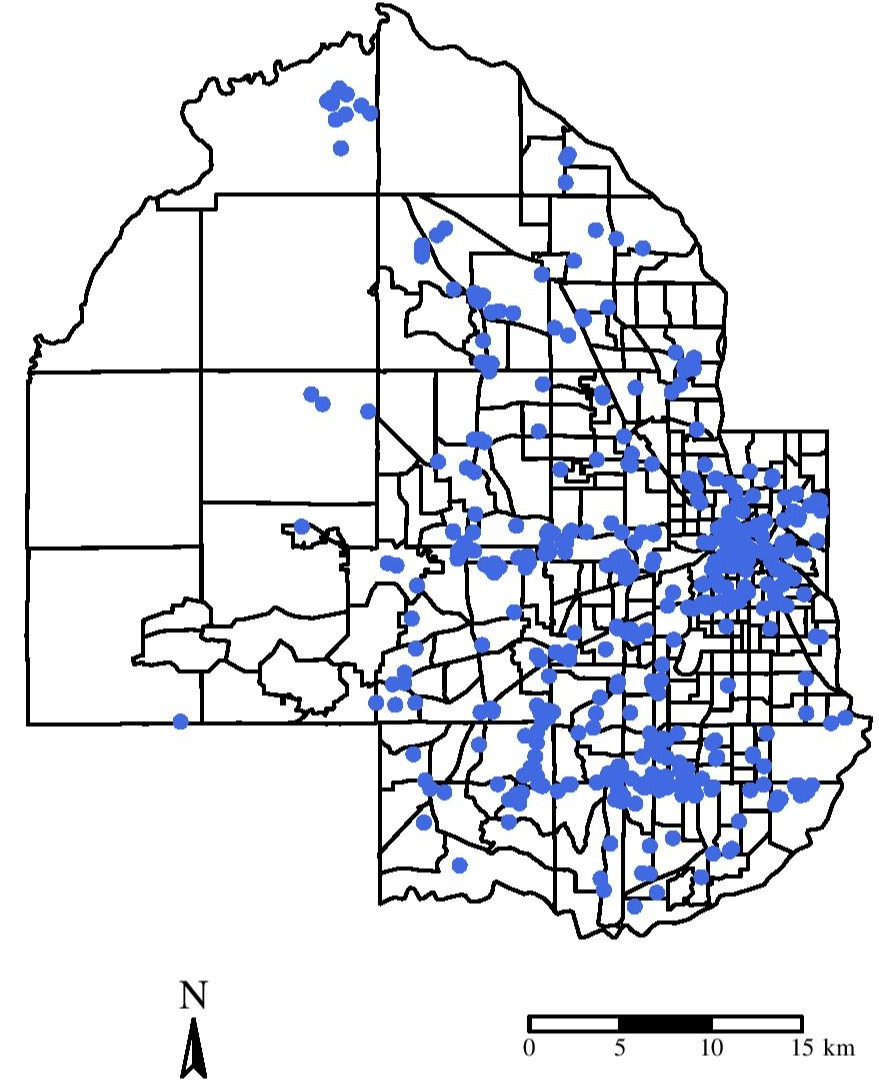
\includegraphics[width = 0.4\textwidth]{hPoints.jpg}
%\end{figure}
%
%\end{frame}


\end{document}